\documentclass{beamer}
\usetheme[compressed]{Singapore}
\useinnertheme{circles}
%\usetheme{Montpellier}
\usepackage[italian]{babel}
\setbeamercolor{background canvas}{bg=background}
\setbeamercolor{section in toc}{fg=template}
\setbeamercolor{subsection in toc}{fg=black}
\setbeamerfont{section in toc}{series=\bfseries,size=\normalsize}
\definecolor{background}{RGB}{255, 255, 255}
\definecolor{royalblue3}{RGB}{58,95,205}
\definecolor{giallo}{RGB}{197, 151, 0}
\definecolor{template}{RGB}{54, 114, 89}
%\definecolor{template}{RGB}{1, 116, 179}
%\definecolor{template}{RGB}{0, 113, 79}
\definecolor{but}{RGB}{181, 18, 27}
%\definecolor{template}{RGB}{181, 18, 27}
\setbeamercolor{section in head/foot}{fg=white, bg=template}
\setbeamercolor{subsection in head/foot}{fg=template, bg=template!20}
\setbeamercolor{subsection in head/foot}{fg=template, bg=template!20}
\setbeamercolor{frametitle}{fg=template, bg = white}
\setbeamercolor{title}{bg = white, fg=template}
\setbeamercolor{author in head/foot}{bg=template, fg=white}
\setbeamercolor{title in head/foot}{bg=template!40, fg=template}
\setbeamercolor{date in head/foot}{bg=template!20, fg=template}
\setbeamercolor{item}{fg=template!20}
\setbeamercolor{caption name}{fg=template}
\usepackage{tikz}
\usetikzlibrary{shapes}
\usetikzlibrary{plotmarks}
\setbeamerfont{section in toc}{series=\bfseries,size=\normalsize}
\setbeamerfont{title}{family=\scshape}
\usepackage{tikzsymbols}
\usetikzlibrary{mindmap,calc,patterns,decorations.pathmorphing,decorations.markings, arrows, shapes.arrows, shapes, backgrounds,positioning,shadows.blur, positioning, fit, tikzmark}
\usepackage{multirow}
\usepackage{tabularx}
\usepackage{setspace}
\usepackage{booktabs}
\usepackage{tikz}
\usepackage{mathtools}
\usepackage{atbegshi}
\usepackage{amsmath}
\usepackage[symbol]{footmisc}

\tikzset{type1/.style={circle, fill=blue},
	type2/.style={circle, fill=red},
	type3/.style={circle, fill=olive},
	type4/.style={circle, fill=cyan},
	type5/.style={circle, fill=giallo},
	type6/.style={circle, fill=blu},
	info/.style = {rectangle, rounded corners, minimum width=1.5cm, minimum height=10cm, text centered, draw=white,  text width=5.5cm},
	stat/.style = {rectangle, minimum width=1.5cm, minimum height=10cm, text justified, draw=white,  text width=5.5cm}
}

\usepackage[absolute,overlay]{textpos}
\newcommand\Factor{1.2}

\renewcommand*{\thefootnote}{\fnsymbol{footnote}}


\tikzset{type1/.style={circle, fill=template},
	type2/.style={circle, fill=red},
		type3/.style={circle, fill=olive},
			type4/.style={circle, fill=cyan},
				type5/.style={circle, fill=giallo},
					type6/.style={circle, fill=template},
	info/.style = {rectangle, rounded corners, minimum width=2.5cm, minimum height=0.1cm, text centered, draw=black,  text width=2.5cm},
	stat/.style = {rectangle, rounded corners, minimum width=2.5cm, minimum height=0.1cm, text centered, draw=white,  text width=2.5cm}
}

\AtBeginSection[]
{
	\begin{frame}
		\tableofcontents[currentsection,currentsubsection]
	\end{frame}
}  

\AtBeginSubsection[]
{
	\begin{frame}
		\tableofcontents[currentsection,currentsubsection]
	\end{frame}
}  

\AtBeginSubsubsection[]
{
	\begin{frame}
		\tableofcontents[currentsection,currentsubsection]
	\end{frame}
}  

\newcommand{\tstar}[5]{% inner radius, outer radius, tips, rot angle, options
	\pgfmathsetmacro{\starangle}{360/#3}
	\draw[#5] (#4:#1)
	\foreach \x in {1,...,#3}
	{ -- (#4+\x*\starangle-\starangle/2:#2) -- (#4+\x*\starangle:#1)
	}
	-- cycle;
}

\newcommand{\ngram}[4]{% outer radius, tips, rot angle, options
	\pgfmathsetmacro{\starangle}{360/#2}
	\pgfmathsetmacro{\innerradius}{#1*sin(90-\starangle)/sin(90+\starangle/2)}
	\tstar{\innerradius}{#1}{#2}{#3}{#4}
}

 \tikzset{
	invisible/.style={opacity=0},
	visible on/.style={alt={#1{}{invisible}}},
	alt/.code args={<#1>#2#3}{%
		\alt<#1>{\pgfkeysalso{#2}}{\pgfkeysalso{#3}} % \pgfkeysalso doesn't change the path
	},
	every overlay node/.style={
		%draw=black,fill=white,rounded corners,
		anchor=north west, inner sep=0pt,
	},
}

\def\tikzoverlay{%
	\tikz[remember picture, overlay]\node[every overlay node]
}%

%\setbeamertemplate{section page}
%{
%	\begingroup
%	\begin{beamercolorbox}[sep=12pt,center]{section title}
%		\usebeamerfont{section title}\insertsection\par
%	\end{beamercolorbox}
%	\endgroup
%}




\title[Questionnaires and Beyond]{Questionnaires and beyond: \\ The Rasch model
}
\institute[]{September 28\textsuperscript{th} 2022, Padova}
\author[]{\texorpdfstring{Ottavia M. Epifania\newline\url{ottavia.epifania@unipd.it} \newline Univerisity of  Padova \newline Catholic University of the Sacred Heart}{Author}}
\date{XXX Conference of the Italian Association of Psychology (AIP)}
\titlegraphic{%
	
\includegraphics[width=1.8cm,height=1.8cm,keepaspectratio]{unipd.png}%\hspace*{9.75cm}~%
	
\includegraphics[width=2.5cm,height=2.5cm,keepaspectratio]{psicostat.png}%
	
\includegraphics[width=1.8cm,height=1.8cm,keepaspectratio]{unicatt.png}%
}
\begin{document}
\begin{frame}[plain]
    \maketitle
\end{frame}

\section{The intuition}

\begin{frame}
	\onslide<1->
	\tikzoverlay (bart) at (-0.8cm,2.2cm) {%
		\begin{minipage}{.20\textwidth}
			\begin{figure}
				\centering
				
\includegraphics[width=\linewidth]{bart.png}
			\end{figure}
		\end{minipage}
	};
	\tikzoverlay (bart1) at (-0.8cm,-1.3cm) {%
		\begin{minipage}{.20\textwidth}
			\centering
			$A_\text{Bart}$
			
		\end{minipage}
	};
	\tikzoverlay (lisa) at (8.5cm,1.5cm) {%
		\begin{minipage}{.20\textwidth}
			\begin{figure}
				\centering
				
\includegraphics[width=\linewidth]{lisa.png}
			\end{figure}
		\end{minipage}
	};
	
	\tikzoverlay (lisa1) at (9.2cm,-0.8cm) {%
		\begin{minipage}{.20\textwidth}
			\centering
			$A_\text{Lisa}$
			
		\end{minipage}
	};
		\onslide<2->
\tikzoverlay (math) at (1.5cm,2.0cm) {%
	\begin{minipage}{.60\textwidth}
\begin{columns}[T]
	\begin{column}{.50\linewidth}
		\centering \textbf{Q1}
		\begin{equation*}
			4 + 5 = ?
		\end{equation*}
	\end{column}

	\begin{column}{.50\linewidth}
		\centering \textbf{Q2}
		\begin{equation*}
			\dfrac{3}{2}x^2 + \dfrac{5}{4}x = ?
		\end{equation*}
\end{column}
\end{columns}
	\end{minipage}
};
\tikzoverlay (math1) at (1.3cm,0.5cm) {%
	\begin{minipage}{.60\textwidth}
		\begin{columns}[T]
			
			\begin{column}{.50\linewidth}
				\begin{equation*}
					d_{q1}
				\end{equation*}
			\end{column}
			\begin{column}{.50\linewidth}
				\begin{equation*}
				d_{q2}
			\end{equation*}
			\end{column}
		\end{columns}
	\end{minipage}
};

\onslide<3->
\tikzoverlay (eq) at (0.3cm, -1.5cm){
\begin{minipage}{.30\linewidth}
	\begin{equation}
		\dfrac{A_p}{d_i}
	\end{equation}
\centering
\vspace{3mm}
$> 1$ if $A_p > d_i$

$< 1$ if $A_p < d_i$
\end{minipage}
};
\tikzoverlay (eq1) at (5.3cm, -1.5cm){
	\begin{minipage}{.50\linewidth}
		\begin{equation}
			P(X_{pi} = 1) = \dfrac{\dfrac{A_p}{d_i}}{1 + \dfrac{A_p}{d_i}}
		\end{equation}
	\end{minipage}
};
\end{frame}

\section{The model}
\begin{frame}
\begin{figure}
	\centering
	
\includegraphics[width=0.5\linewidth]{later}
\end{figure}
\begin{columns}[T]
	\begin{column}{.5\linewidth}
		\centering
		$ln(A_p) = \beta_p$
	\end{column}
	\begin{column}{.5\linewidth}
	\centering
	$ln(d_i) = \delta_i$
\end{column}
\end{columns}

\vspace{3mm}
\begin{equation}
P(X_{pi} = 1|\beta_p, \delta_i) = \dfrac{exp(\beta_p - \delta_i)}{1 + exp(\beta_p - \delta_i)}
\end{equation}
\end{frame}

\begin{frame}

	\begin{overprint}
		\centering
	\onslide<1>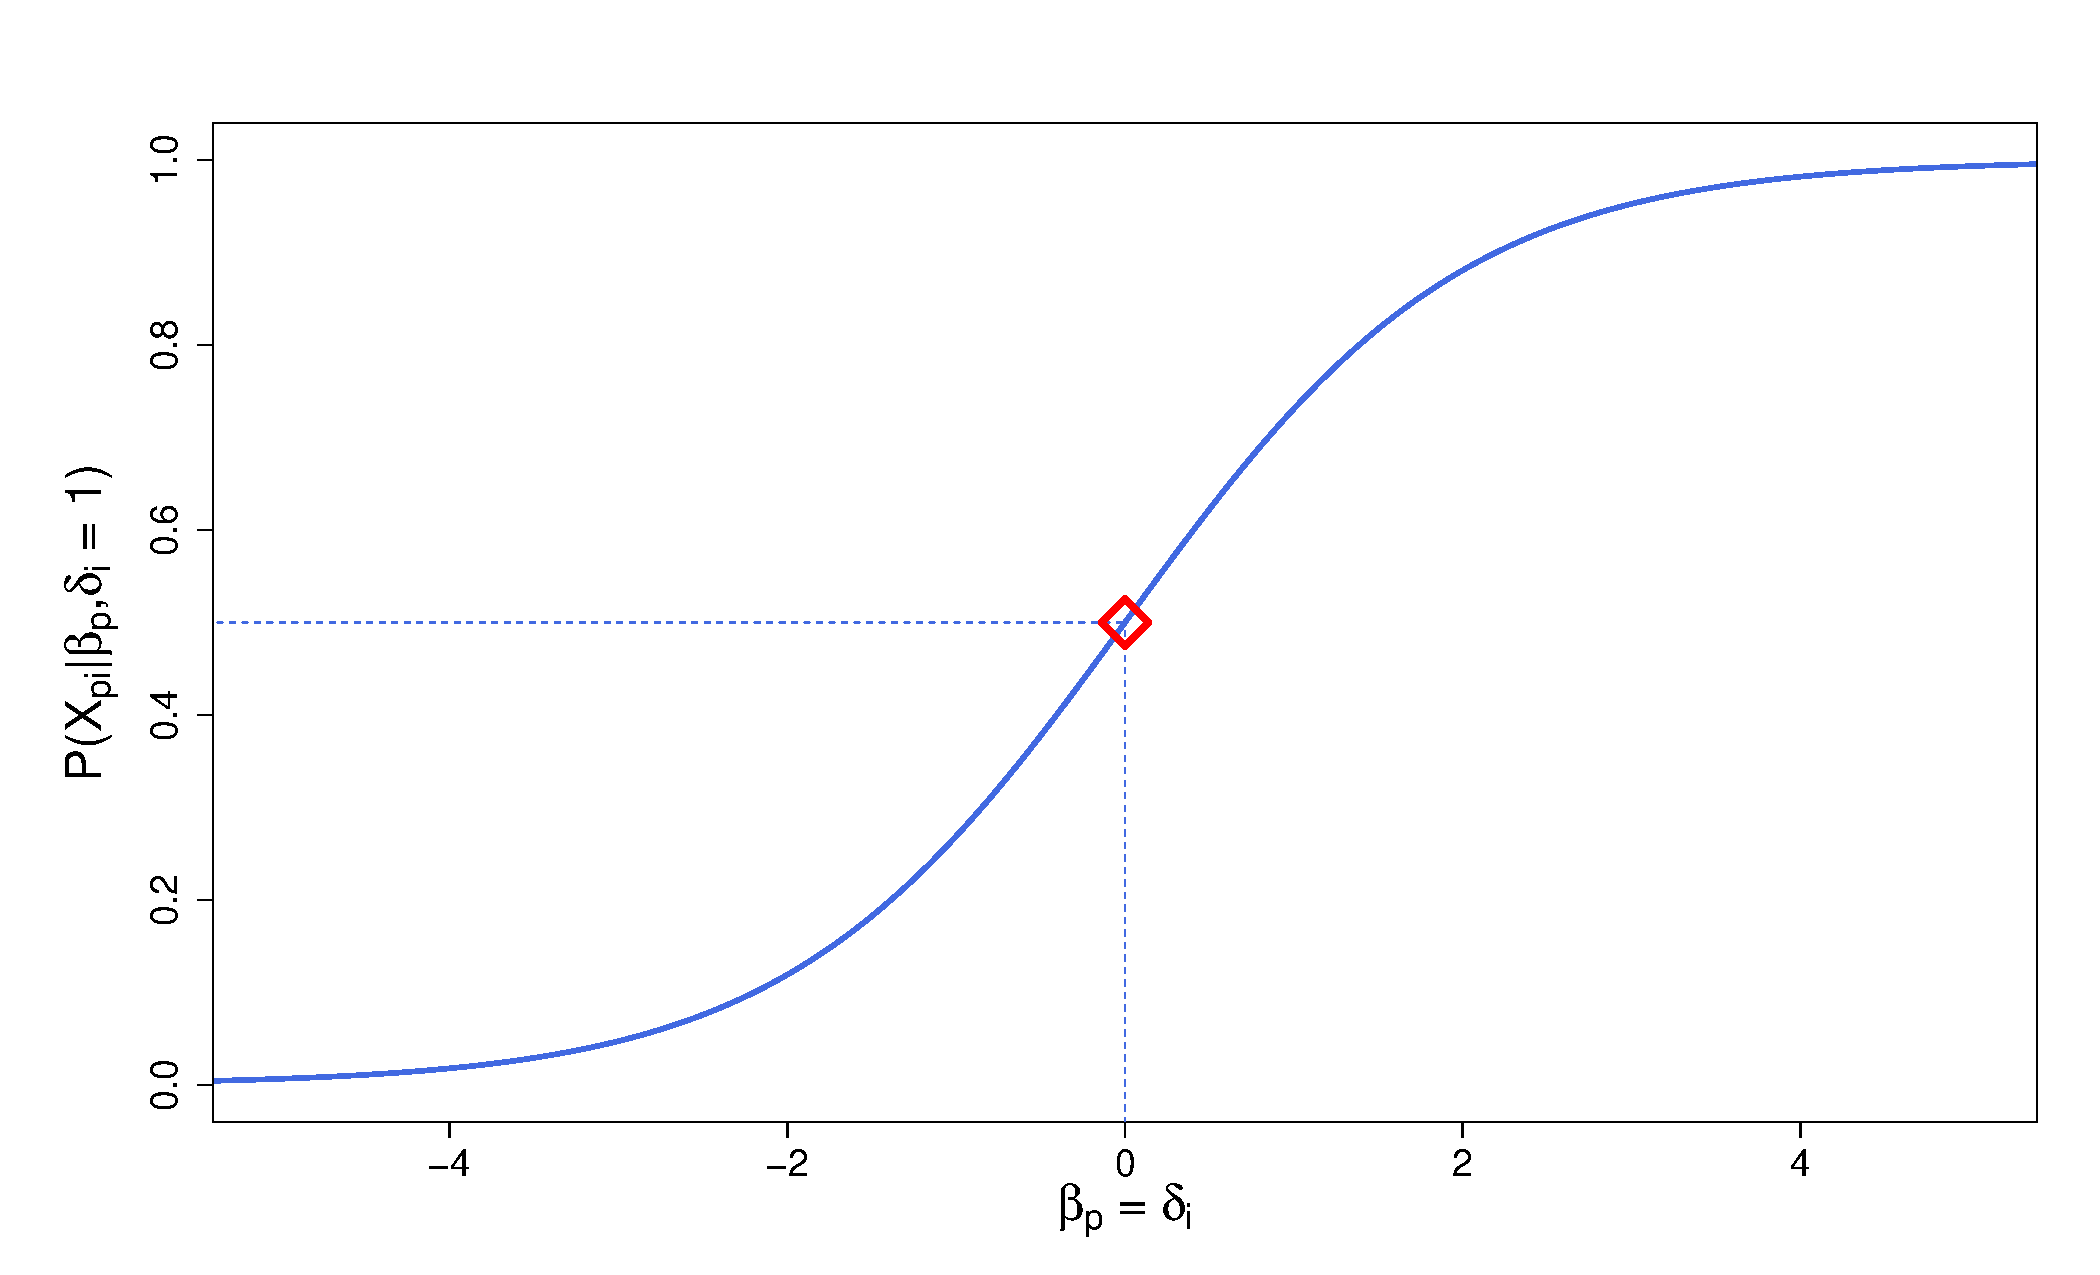
\includegraphics[width=\linewidth]{base.pdf}
	\onslide<2>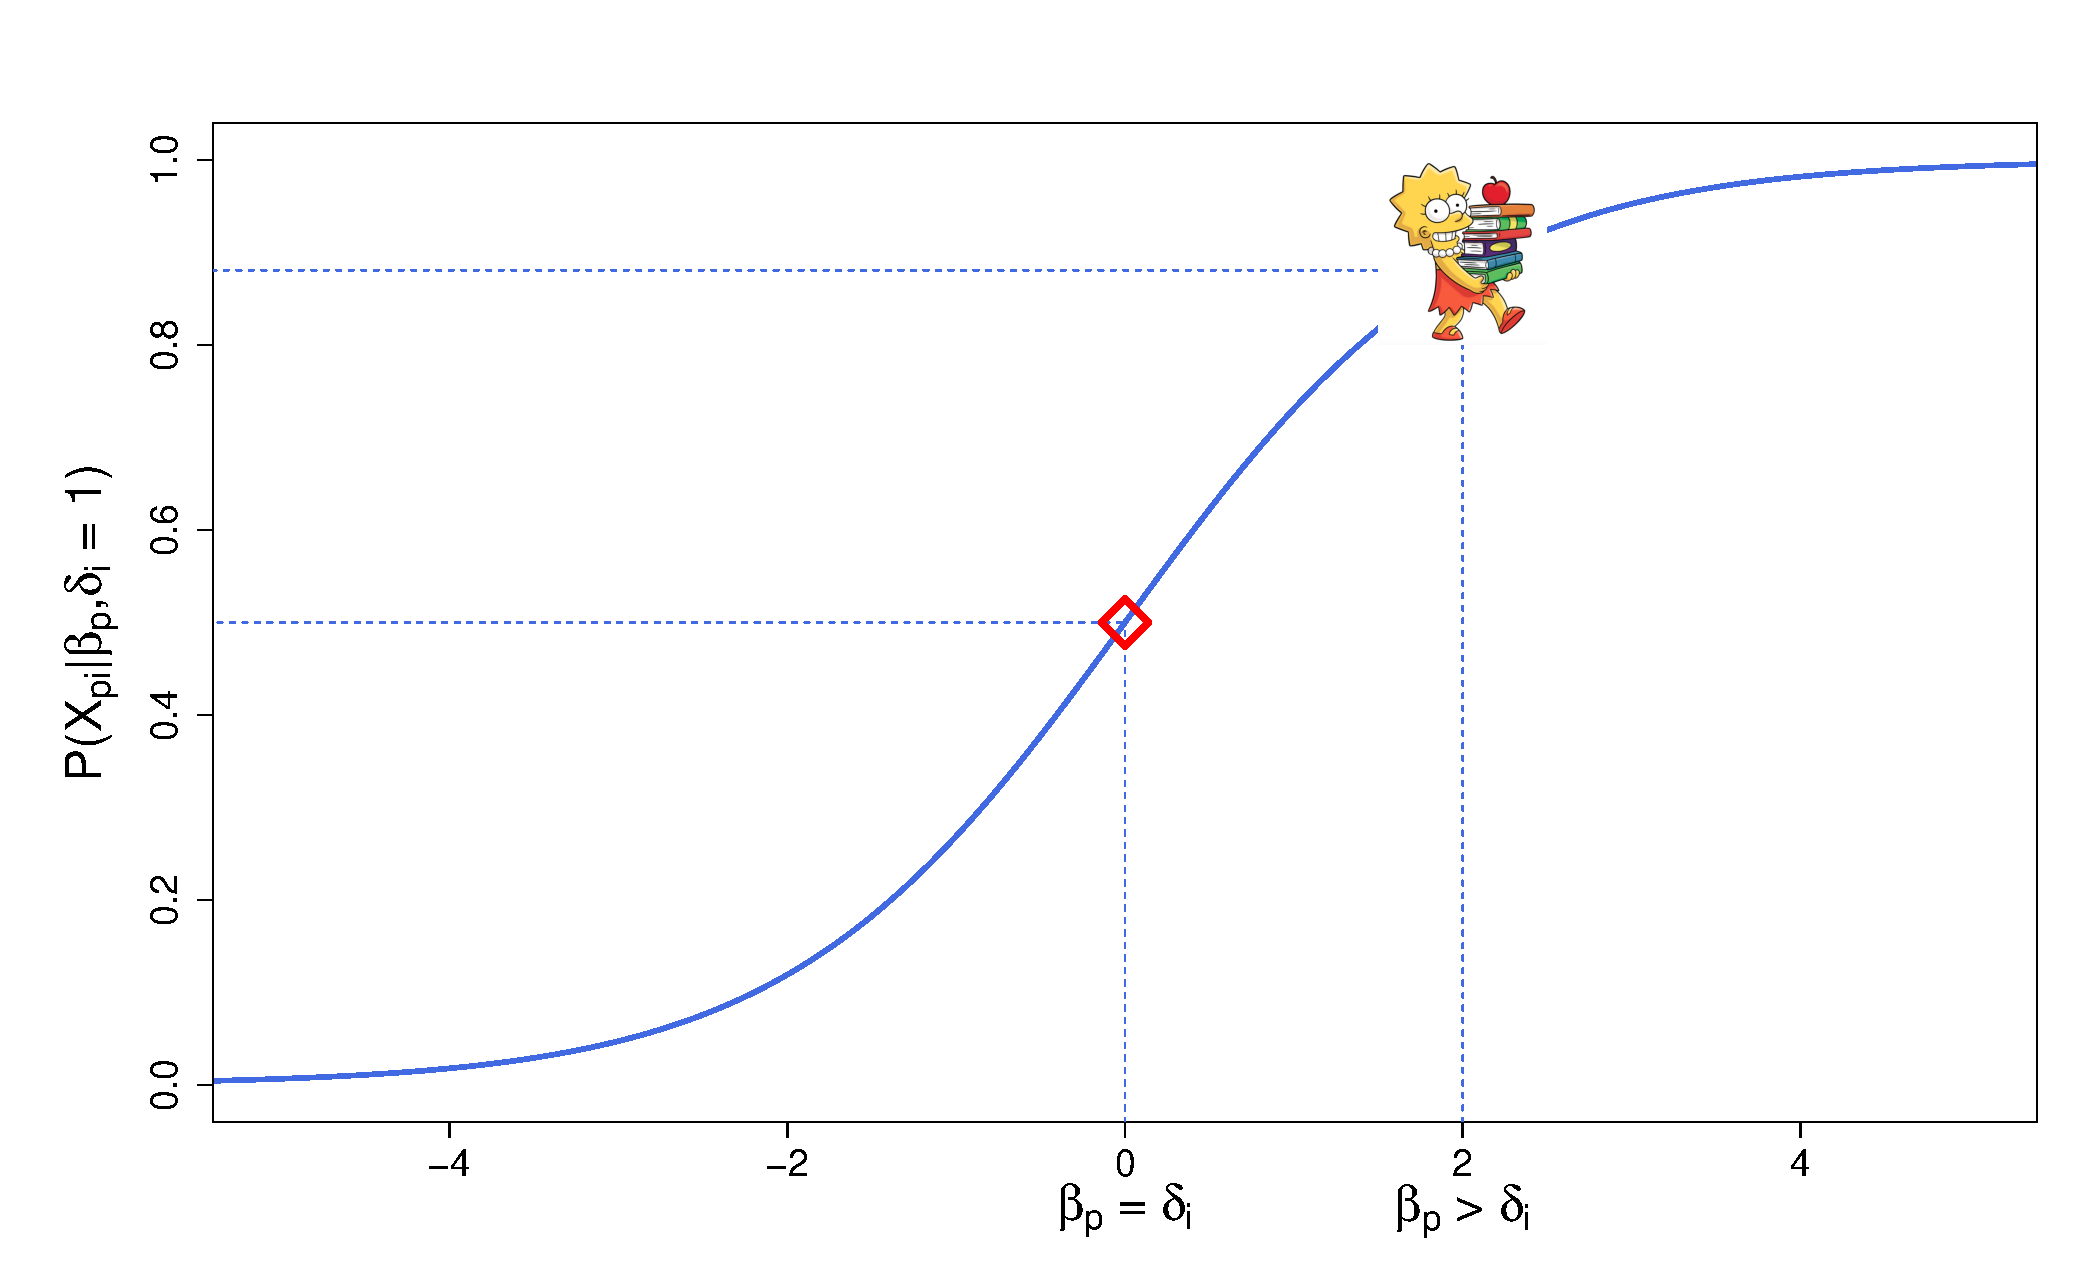
\includegraphics[width=\linewidth]{lisa.pdf}
	\onslide<3>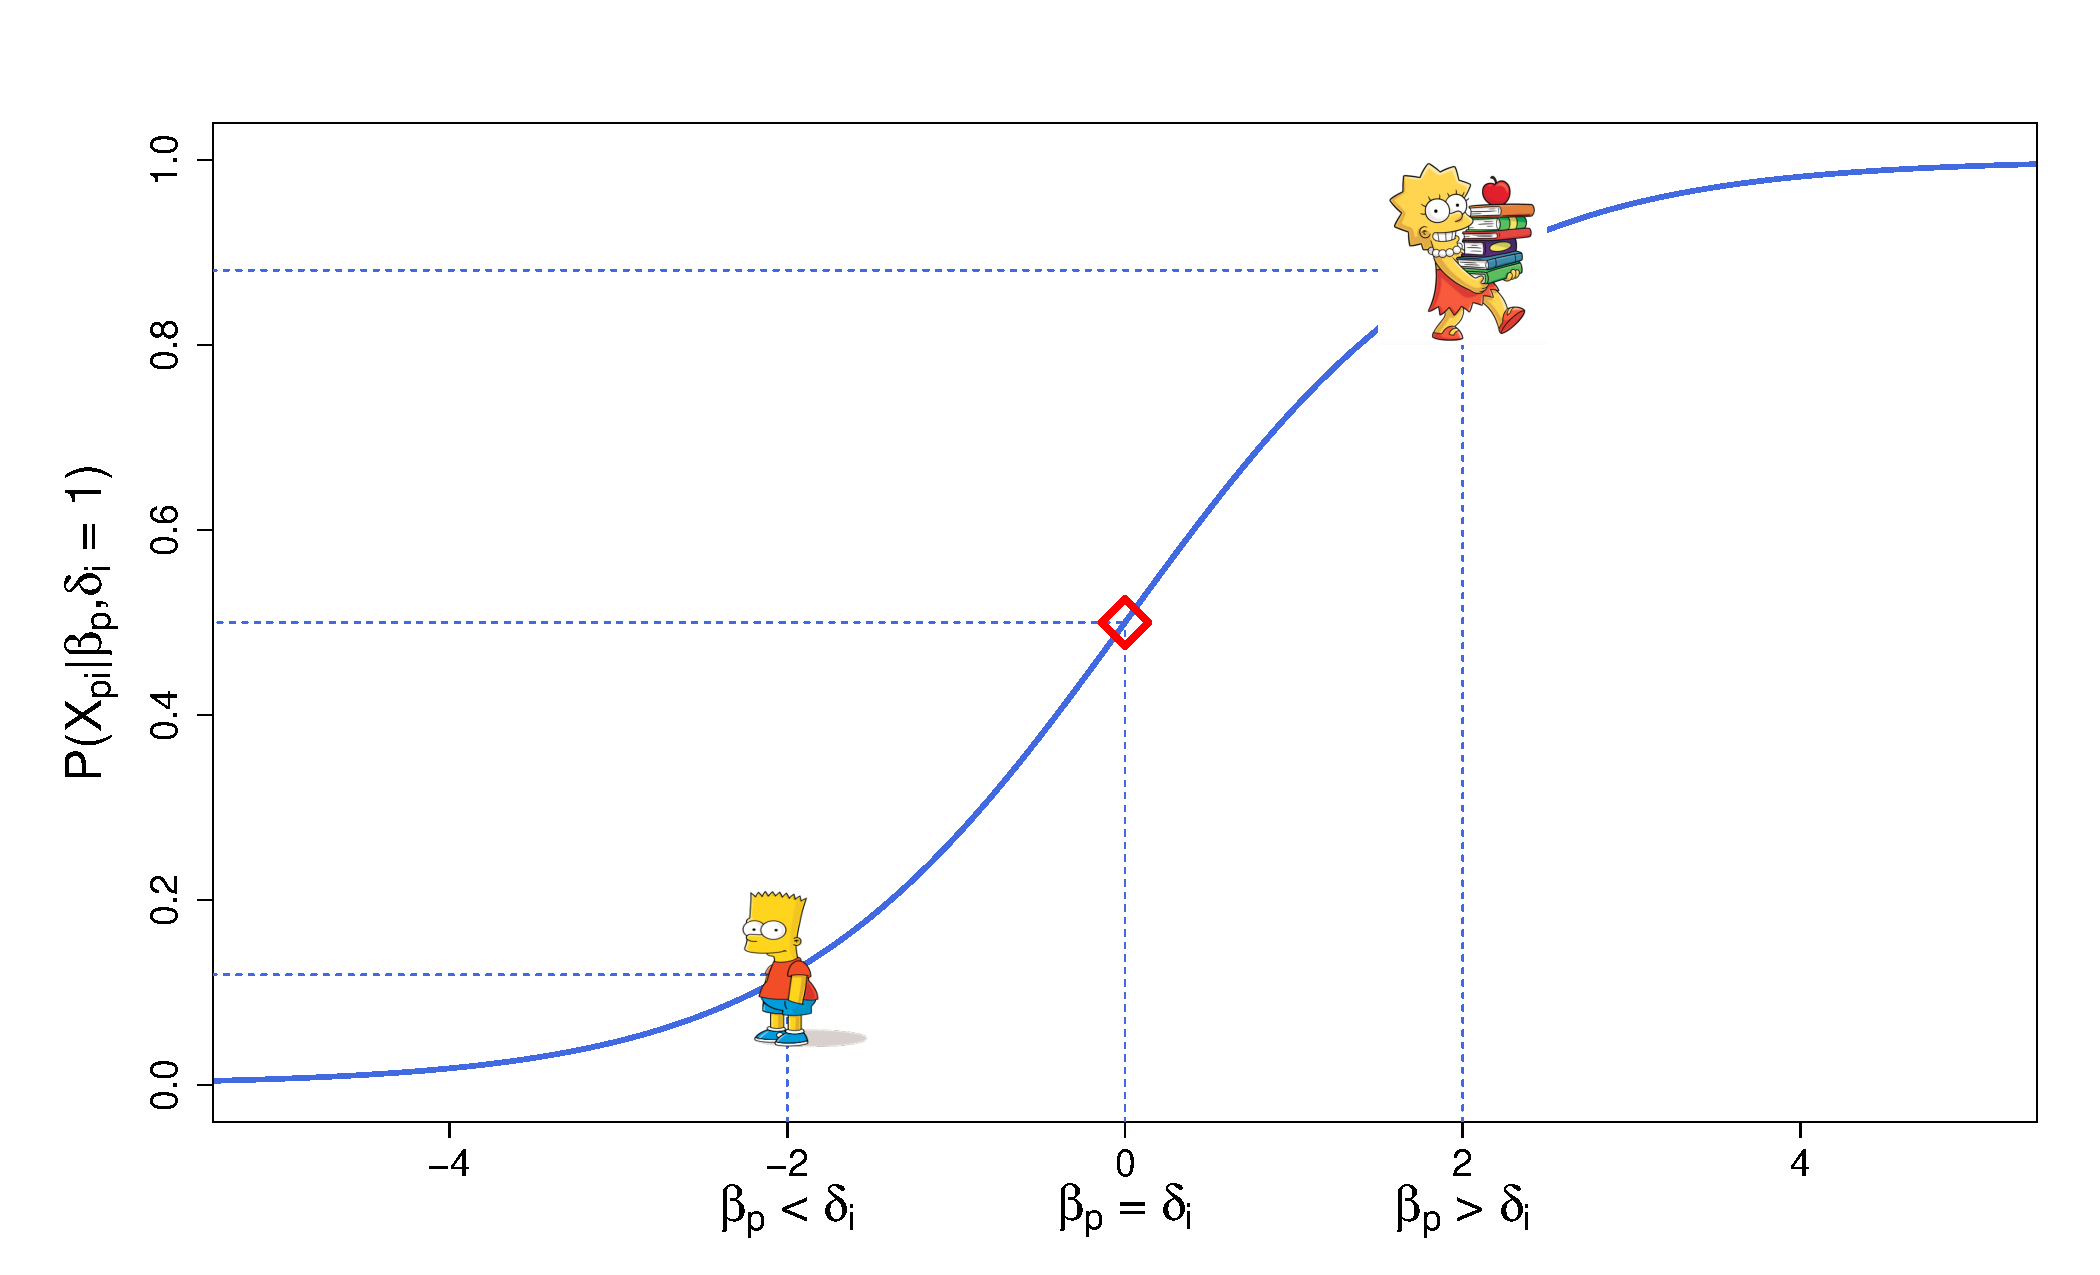
\includegraphics[width=\linewidth]{bart.pdf}
\end{overprint}
\end{frame}


\section{Wait...}

\begin{frame}
\begin{center}
	* Eureka moment *
\end{center}

\begin{figure}
	\centering
	
\includegraphics[width=0.6\linewidth]{psicostat}
\end{figure}


\end{frame}

\begin{frame}

\begin{center}
	Generalized Linear Model (GLM)\\
	\small binomially distributed responses
\end{center}

	\begin{overprint}
					\onslide<2>
					\centering
					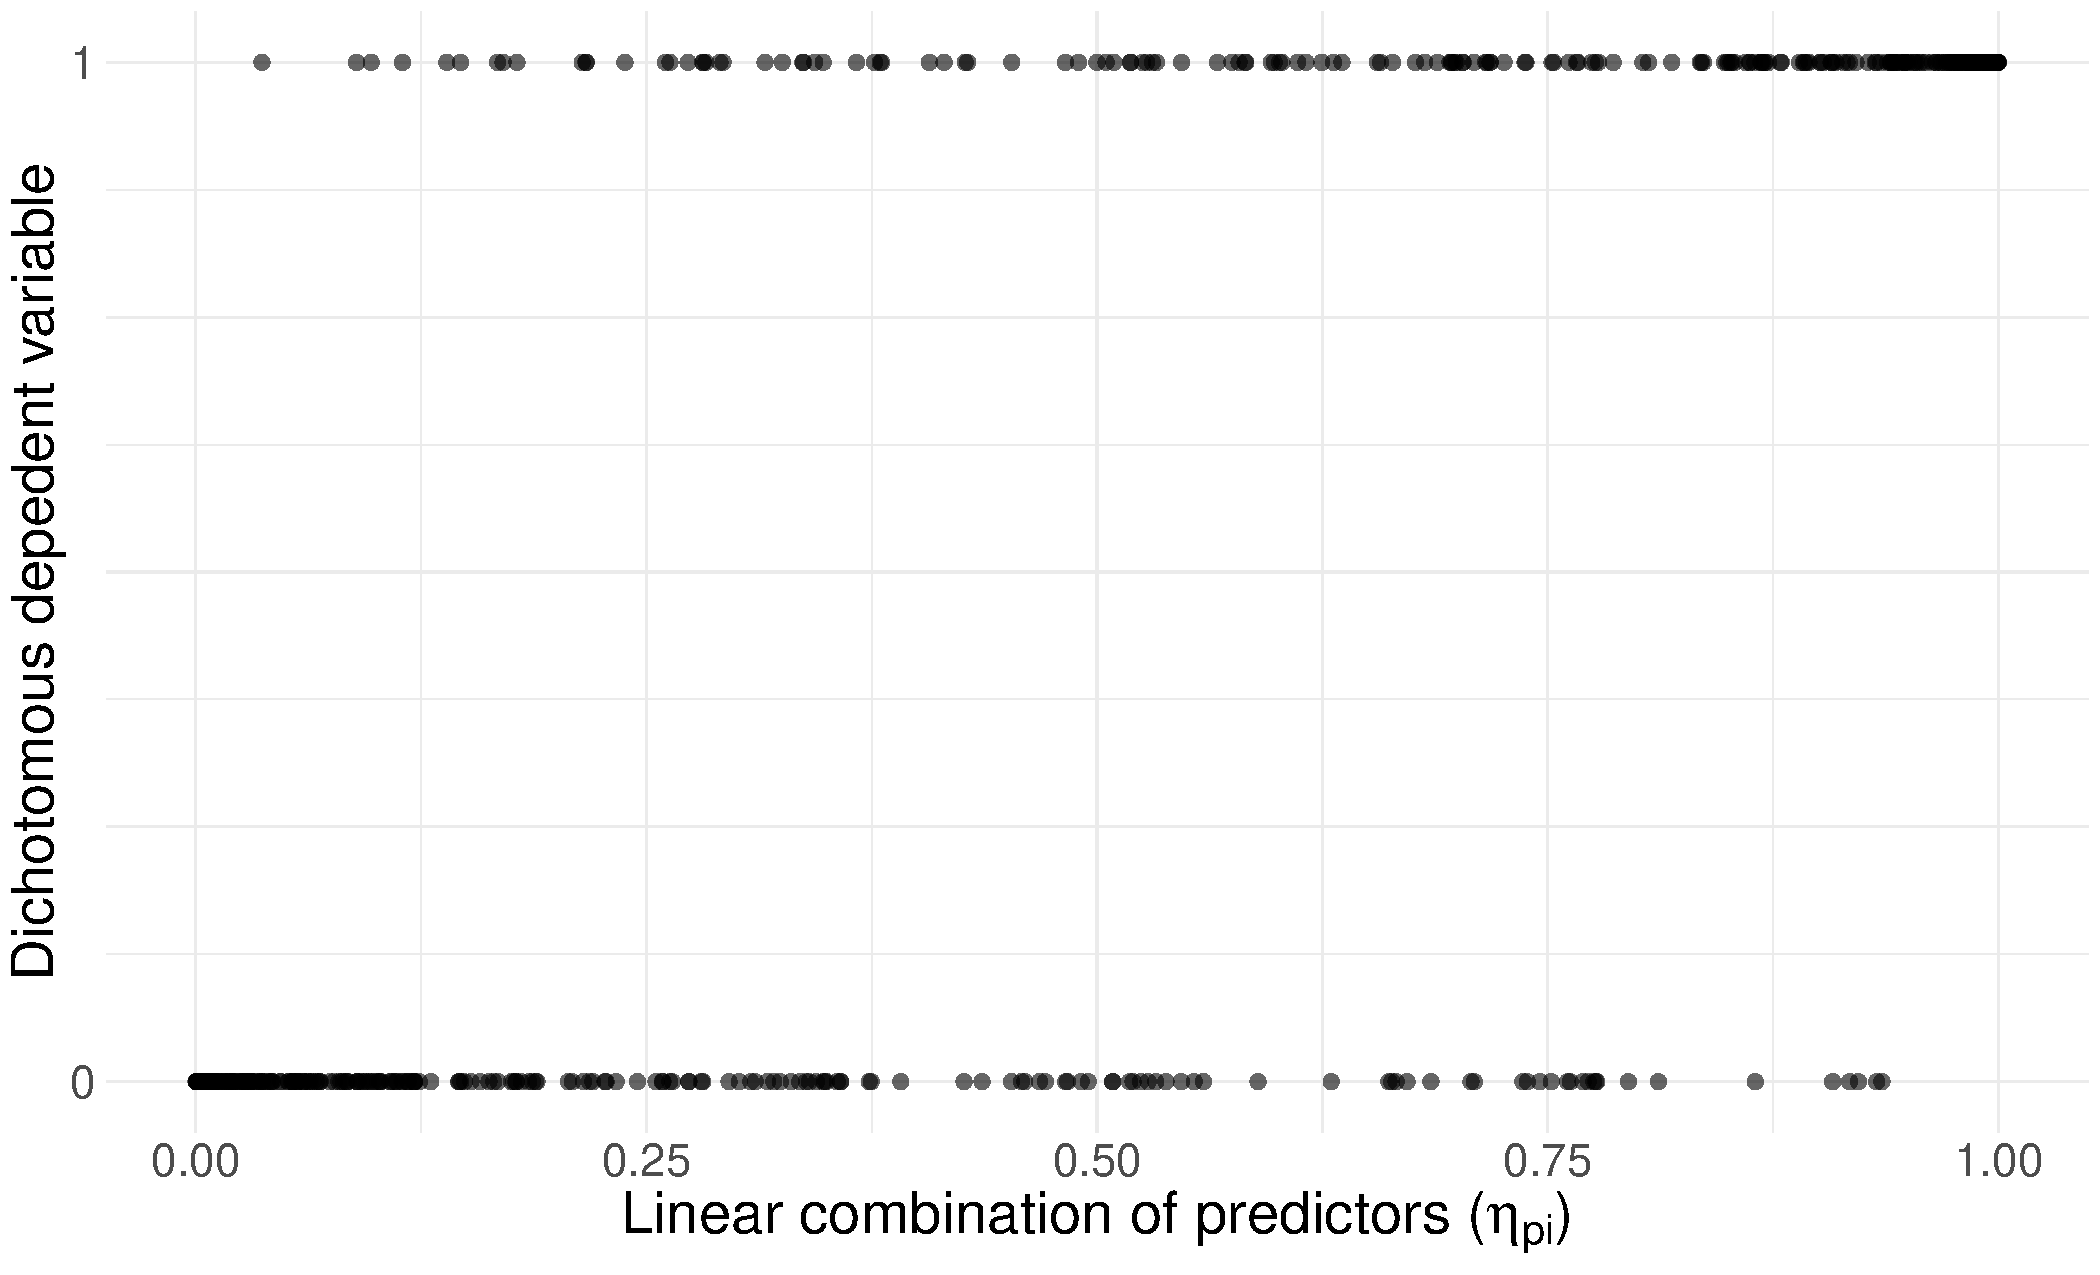
\includegraphics[width=.70\linewidth]{baseGLM.pdf}
			\onslide<3>
				\centering
				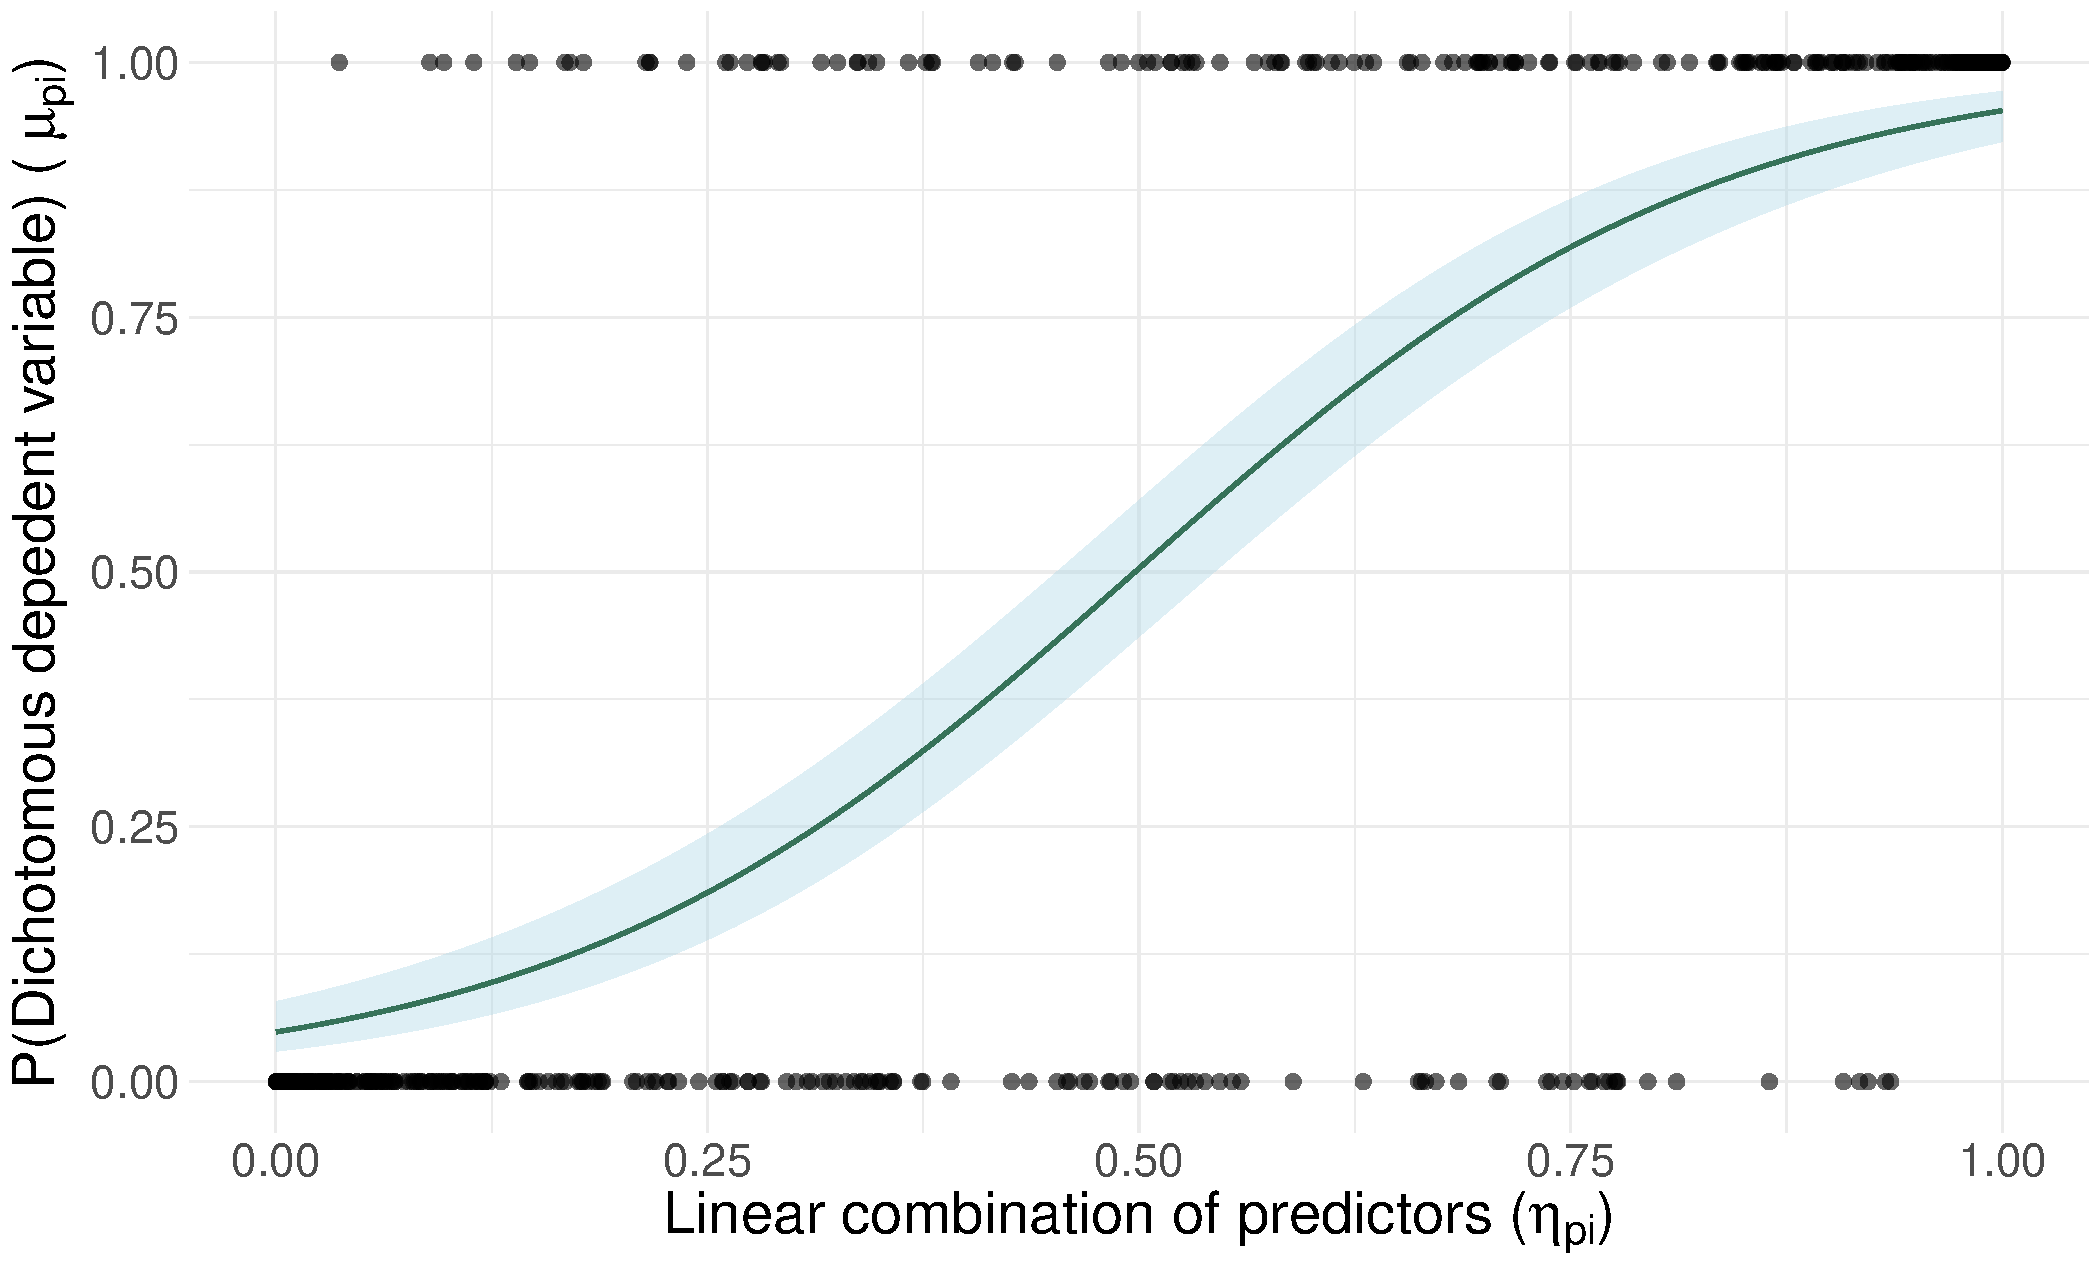
\includegraphics[width=.70\linewidth]{linkGLM.pdf}
	\end{overprint}


\onslide<2->
		\begin{equation*}
	\mu_{pi} = g(\eta_{pi}) = log\left(\frac{\mu_{pi}}{1 - \mu_{pi}}\right)
\end{equation*}

\onslide<3->
\begin{equation*}
	g^{-1} = \frac{exp(\eta_{pi})}{1 + exp(\eta_{pi})}
\end{equation*}
\end{frame}


\section{Why is it useful?}

\begin{frame}
	Rasch model: Dichotomous responses 
	
	\onslide<2->
	\begin{alertblock}{Issue}
		
		Quite limiting in Psychological Research
	\end{alertblock}

\onslide<3->
\vspace{5mm}
(Generalized) Linear Model: ``Any'' kind of response

\onslide<4->
\begin{exampleblock}{e.g.: Response times}
	
	log-transformation and log-normal model parametrization
\end{exampleblock} 
\end{frame}



\begin{frame}
	
	\tikzoverlay (prova) at (-1.5cm,2.5cm) {
		\begin{overprint}
		\onslide<1>
		\begin{tikzpicture}[
		elli/.style={ellipse,text width=10cm,align=center,
			minimum height=4cm,inner xsep=-1em,inner ysep=-1em,draw=template}]
		\node[elli] (first) {		\begin{itemize}
				\item \textbf{\textcolor{template}{Linearity of the scores}}
				\begin{quote}
					Logarithm transformation $\rightarrow$ Respondents and items on the same latent trait
				\end{quote}
				\item \textbf{\textcolor{template}{Comparison invariance}}
				\begin{quote}
					Respondents can be compared between each other without considering the items....and vice versa!
				\end{quote}
				\large
				\item \textbf{\textcolor{template}{Local independence}}
				\begin{quote}
					Given the person $\rightarrow$ The responses to the items are independent 	
				\end{quote}
			\end{itemize}
		};
	\end{tikzpicture}
		
		
		\onslide<2>
		\begin{tikzpicture}[
			elli/.style={ellipse,text width=10cm,align=center,
				minimum height=4cm,inner xsep=-1em,inner ysep=-1em,draw=template}]
			\node[elli] (first) {		\begin{itemize}
					\item \textbf{\textcolor{template}{Linearity of the scores}}
					\begin{quote}
						Logarithm transformation $\rightarrow$ Respondents and items on the same latent trait
					\end{quote}
					\item \textbf{\textcolor{template}{Comparison invariance}}
					\begin{quote}
						Respondents can be compared between each other without considering the items....and vice versa!
					\end{quote}
					\large
					\item \LARGE \textbf{\textcolor{template}{Local independence}}
					\begin{quote}
						Given the person $\rightarrow$ The responses to the items are independent 	
					\end{quote}
				\end{itemize}
			};
		\end{tikzpicture}
	\end{overprint}
}; 
\onslide<1>
\tikzoverlay (uni) at (-0.5cm,-3.5cm) {
	\large
\textcolor{template}{\textbf{Unidimensionality}}
};

\end{frame}

\begin{frame}
	\centering
			\begin{tabular}{l l l l l l l l}
		& \multicolumn{3}{c}{Condition A} & & \multicolumn{3}{c}{Condition B}\\
		Giorgio & \Cat[2] & \Snowman[2] & \BasicTree[2]{black!80}{gray!50}{gray!40}{leaf} & & \Cat[2] & \Snowman[2] & \BasicTree[2]{black!80}{gray!50}{gray!40}{leaf} \\
		Giulia & \Cat[2] & \Snowman[2] & \BasicTree[2]{black!80}{gray!50}{gray!40}{leaf} & & \Cat[2] & \Snowman[2] & \BasicTree[2]{black!80}{gray!50}{gray!40}{leaf} \\
		Jessica & \Cat[2] & \Snowman[2] & \BasicTree[2]{black!80}{gray!50}{gray!40}{leaf} & & \Cat[2] & \Snowman[2] &\BasicTree[2]{black!80}{gray!50}{gray!40}{leaf}\\
	\end{tabular}

\vspace{5mm}
\onslide<2->

\NiceReapey[2] \textbf{\textcolor{template}{Local independence}}


\begin{columns}[T]
	\begin{column}{.50\linewidth}
		\onslide<3->
		\begin{center}
			Rasch model
		\end{center}
		\onslide<4->
		\begin{itemize}
			\item Can't  be applied
			\item The estimates would make no sense
		\end{itemize}
	\end{column}

	\begin{column}{.50\linewidth}
		\onslide<3->
	\begin{center}
	Generalized Linear Model
	\end{center}
	\onslide<4->
	\begin{itemize}
		\item Add the random part (Go Mixed)
		\item Obtain a Rasch-like parametrization of the data
	\end{itemize}
\end{column}
\end{columns}


\end{frame}

\section{Closing time}
\begin{frame}
	
	\begin{center}
\Large
		Think outside of the box!
	\end{center}
\vspace{2mm}
\begin{columns}[T] % align columns
	\begin{column}{.50\textwidth}
		\color{template}\rule{\linewidth}{4pt}
		\begin{center}
			\large{Yes}
		\end{center}
	\normalcolor

		Rasch estimates 
		

		\vspace{1.5mm}
		The sky is the limit
		

			\vspace{1.5mm}
		Keep it maximal
	\end{column}%
	\hfill%
	\begin{column}{.50\textwidth}

		\color{but}\rule{\linewidth}{4pt}
		\begin{center}
			\large{But}
		\end{center}
	\normalcolor

		 Rasch-like parametrization
		 
		 	\vspace{1.5mm}
		 Don't over complicate things 
		 

		 	\vspace{1.5mm}
		 Keep it minimal
	\end{column}%
\end{columns}  

	
\pause
	\centering
	\begin{tikzpicture}
		\node (img) {
\includegraphics[width =.30\linewidth]{pesce}};
		\draw[red, line width=1.4mm] 
		(img.south west) -- (img.north east)
		(img.south east) -- (img.north west);
	\end{tikzpicture}
            
\end{frame}

\begin{frame}[plain]
	\begin{figure}
		\centering
		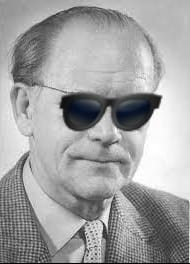
\includegraphics[width=0.5\linewidth]{raschJ}
	\end{figure}
	
	
	\begin{center}
\Huge

\textcolor{template}{Thank you}
	\end{center}
\end{frame}

\begin{frame}[plain]{Questions!}
\begin{figure}
	\centering
	
\includegraphics[width=0.5\linewidth]{domande-simposio-word}
\end{figure}

\vspace{5mm}
\begin{center}
	\href{https://ottaviae.github.io/AIP2022/Rasch/epifaniaRasch.pdf}{https://ottaviae.github.io/AIP2022/Rasch/epifaniaRasch.pdf}
\end{center}

\end{frame}

\end{document}
